% ============================================================
% V. CẢI TIẾN MÔ HÌNH
% ============================================================
\section{Cải tiến mô hình}

\subsection{Phân tích độ khó dữ liệu trước huấn luyện}
\label{subsec:pretrain_data_analysis}

\begin{frame}{V-A. Bối cảnh và động cơ phân tích tiền huấn luyện}
  \small
  Trước huấn luyện, phân tích định lượng được dùng để ước lượng độ khó nội tại của bài toán phân đoạn nguyên liệu.
  \vspace{0.3em}
  \begin{itemize}
    \item FoodSeg103 là benchmark ingredient-level với $103$ lớp, có tính chất \textit{fine-grained} mạnh.
    \item Nhiều lớp có màu và texture gần nhau, biên mờ, nhiều thành phần chồng lấp trong cùng ảnh.
    \item Mô hình nhẹ như BiSeNet dễ mất chi tiết cục bộ sau downsampling, nhất là vùng biên và lớp nhỏ.
  \end{itemize}
  \vspace{0.3em}
  Bộ chỉ số tiền huấn luyện gồm: độ nghiêm trọng mức ảnh/lớp, quan hệ pixel accuracy--present-class mIoU, sink class, và ma trận nhầm lẫn.
\end{frame}

\begin{frame}{V-A.1 Phân bố độ nghiêm trọng ở mức ảnh và lớp}
  \begin{columns}
    \column{0.5\textwidth}
      \begin{figure}
        \centering
        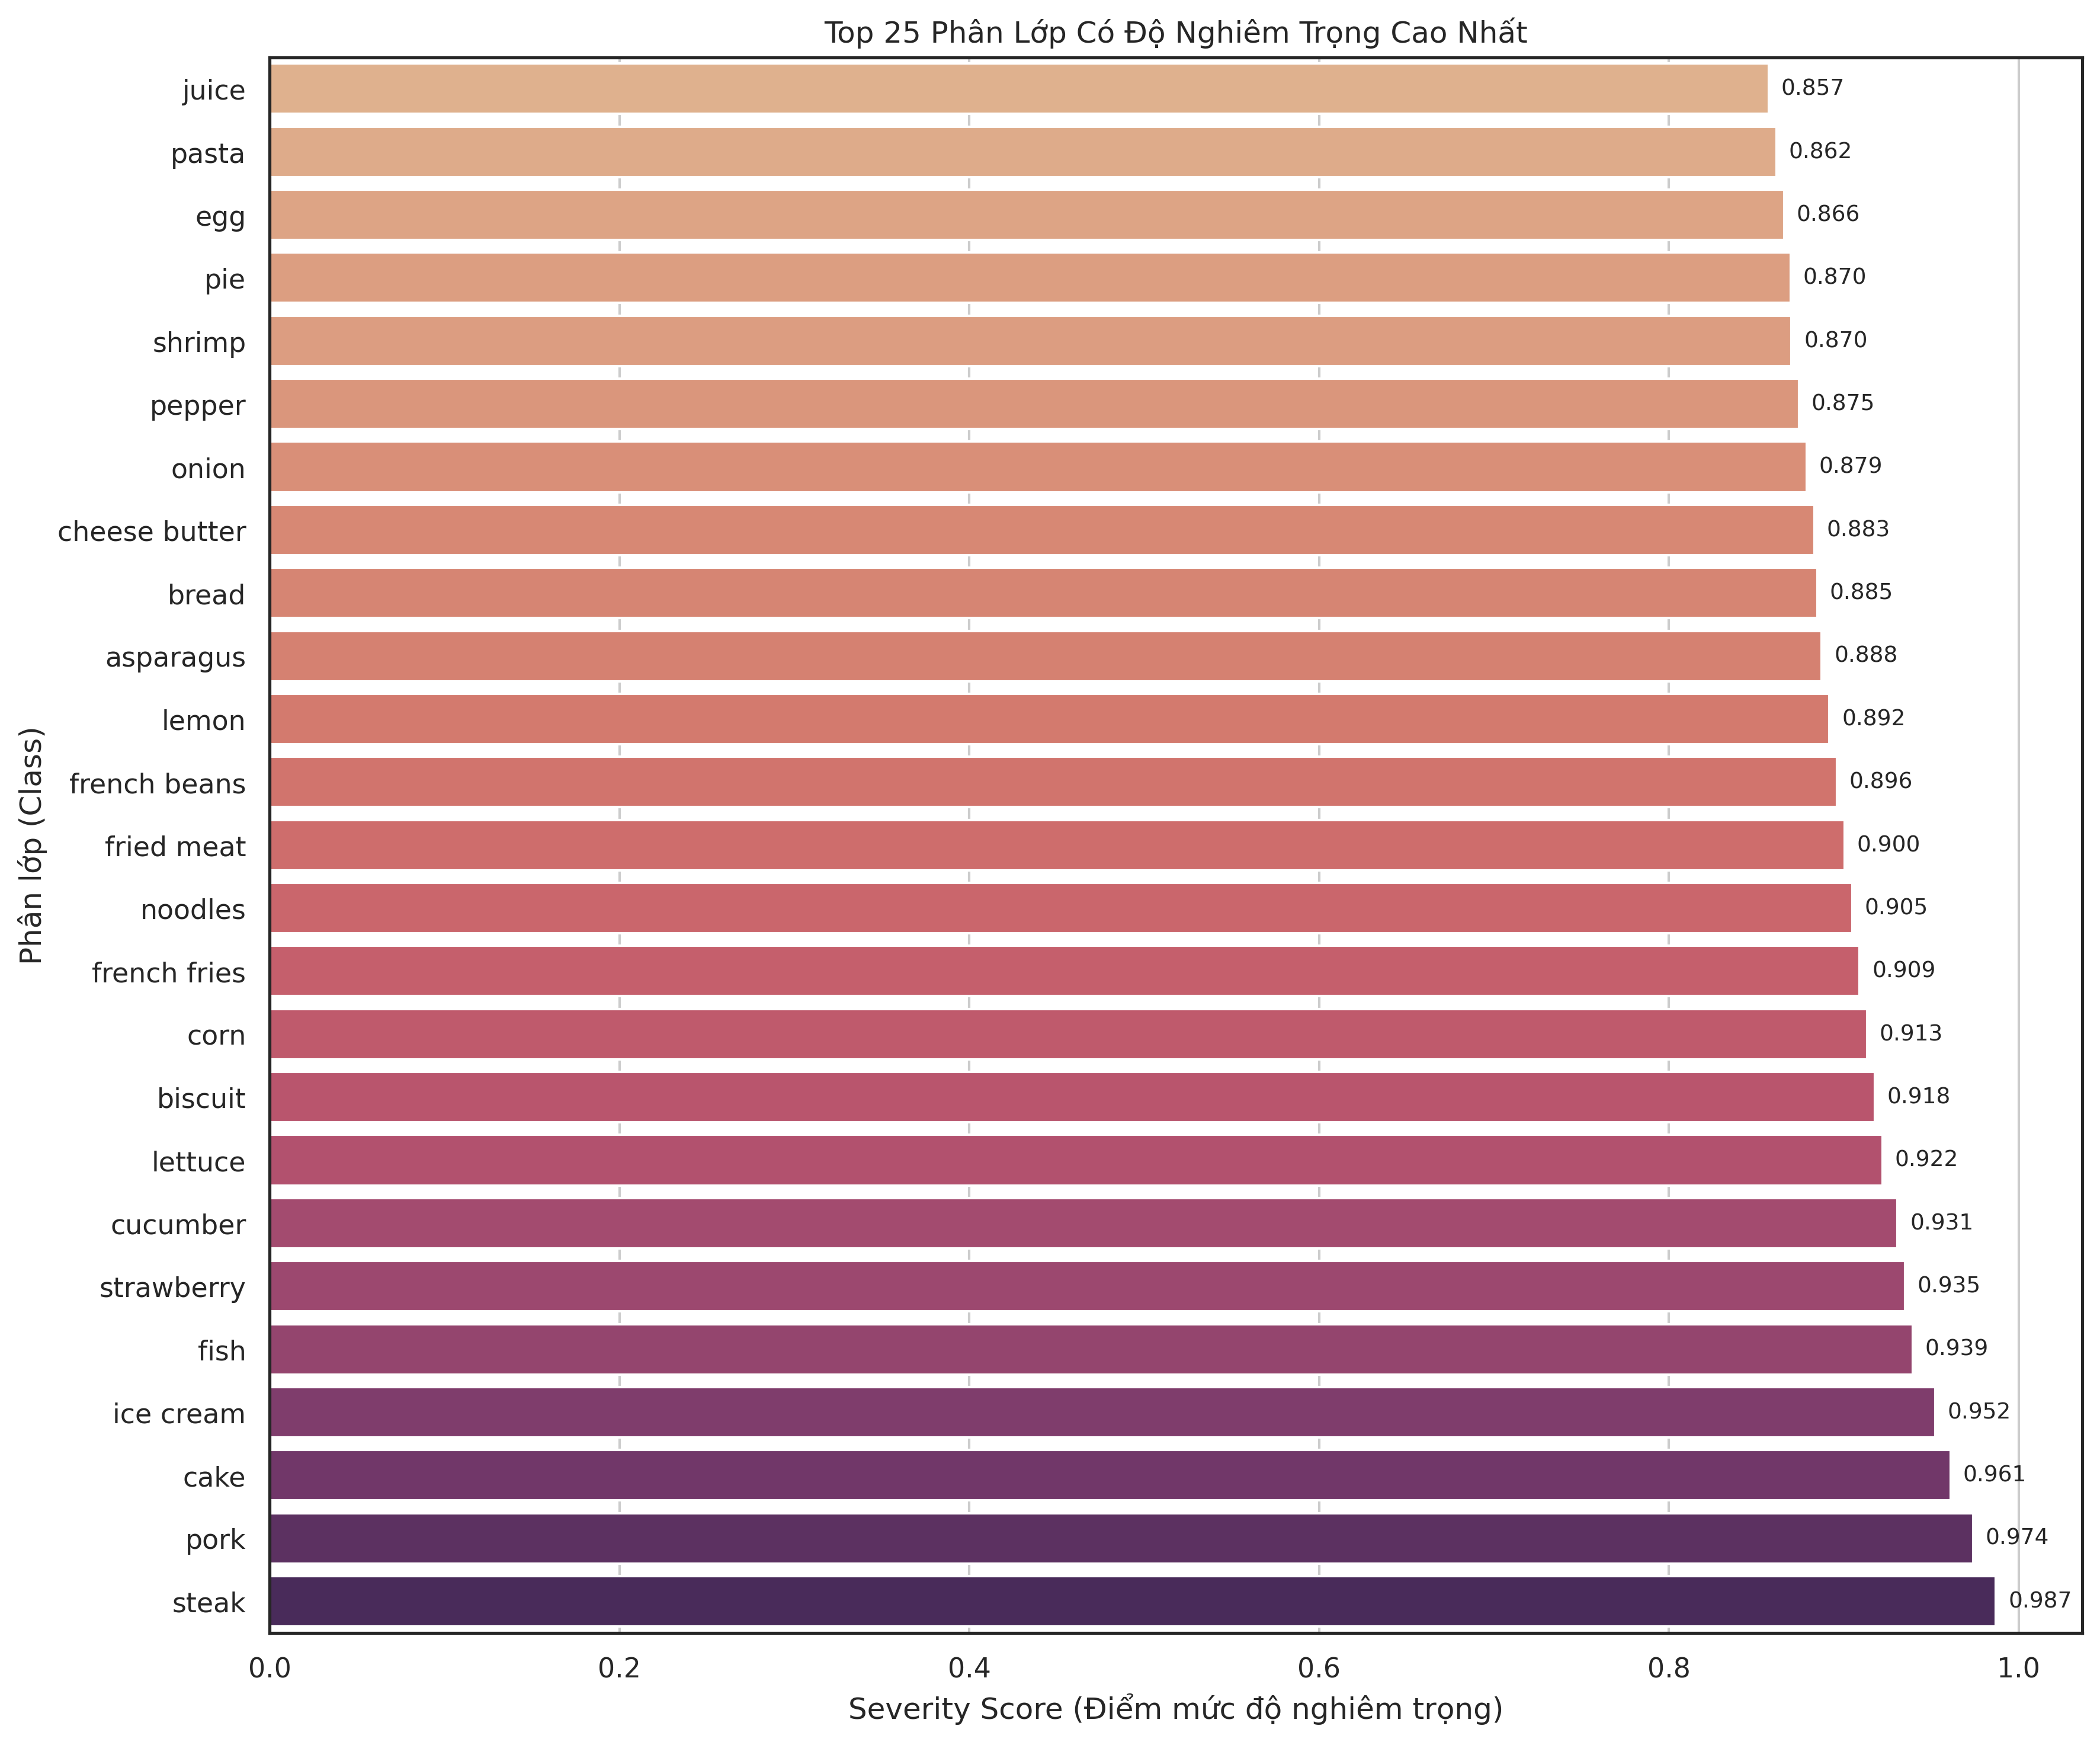
\includegraphics[width=\linewidth]{img/report/caitien/01_class_severity_score_improved.png}
        \caption{Top lớp có điểm severity cao}
      \end{figure}
    \column{0.5\textwidth}
      \begin{figure}
        \centering
        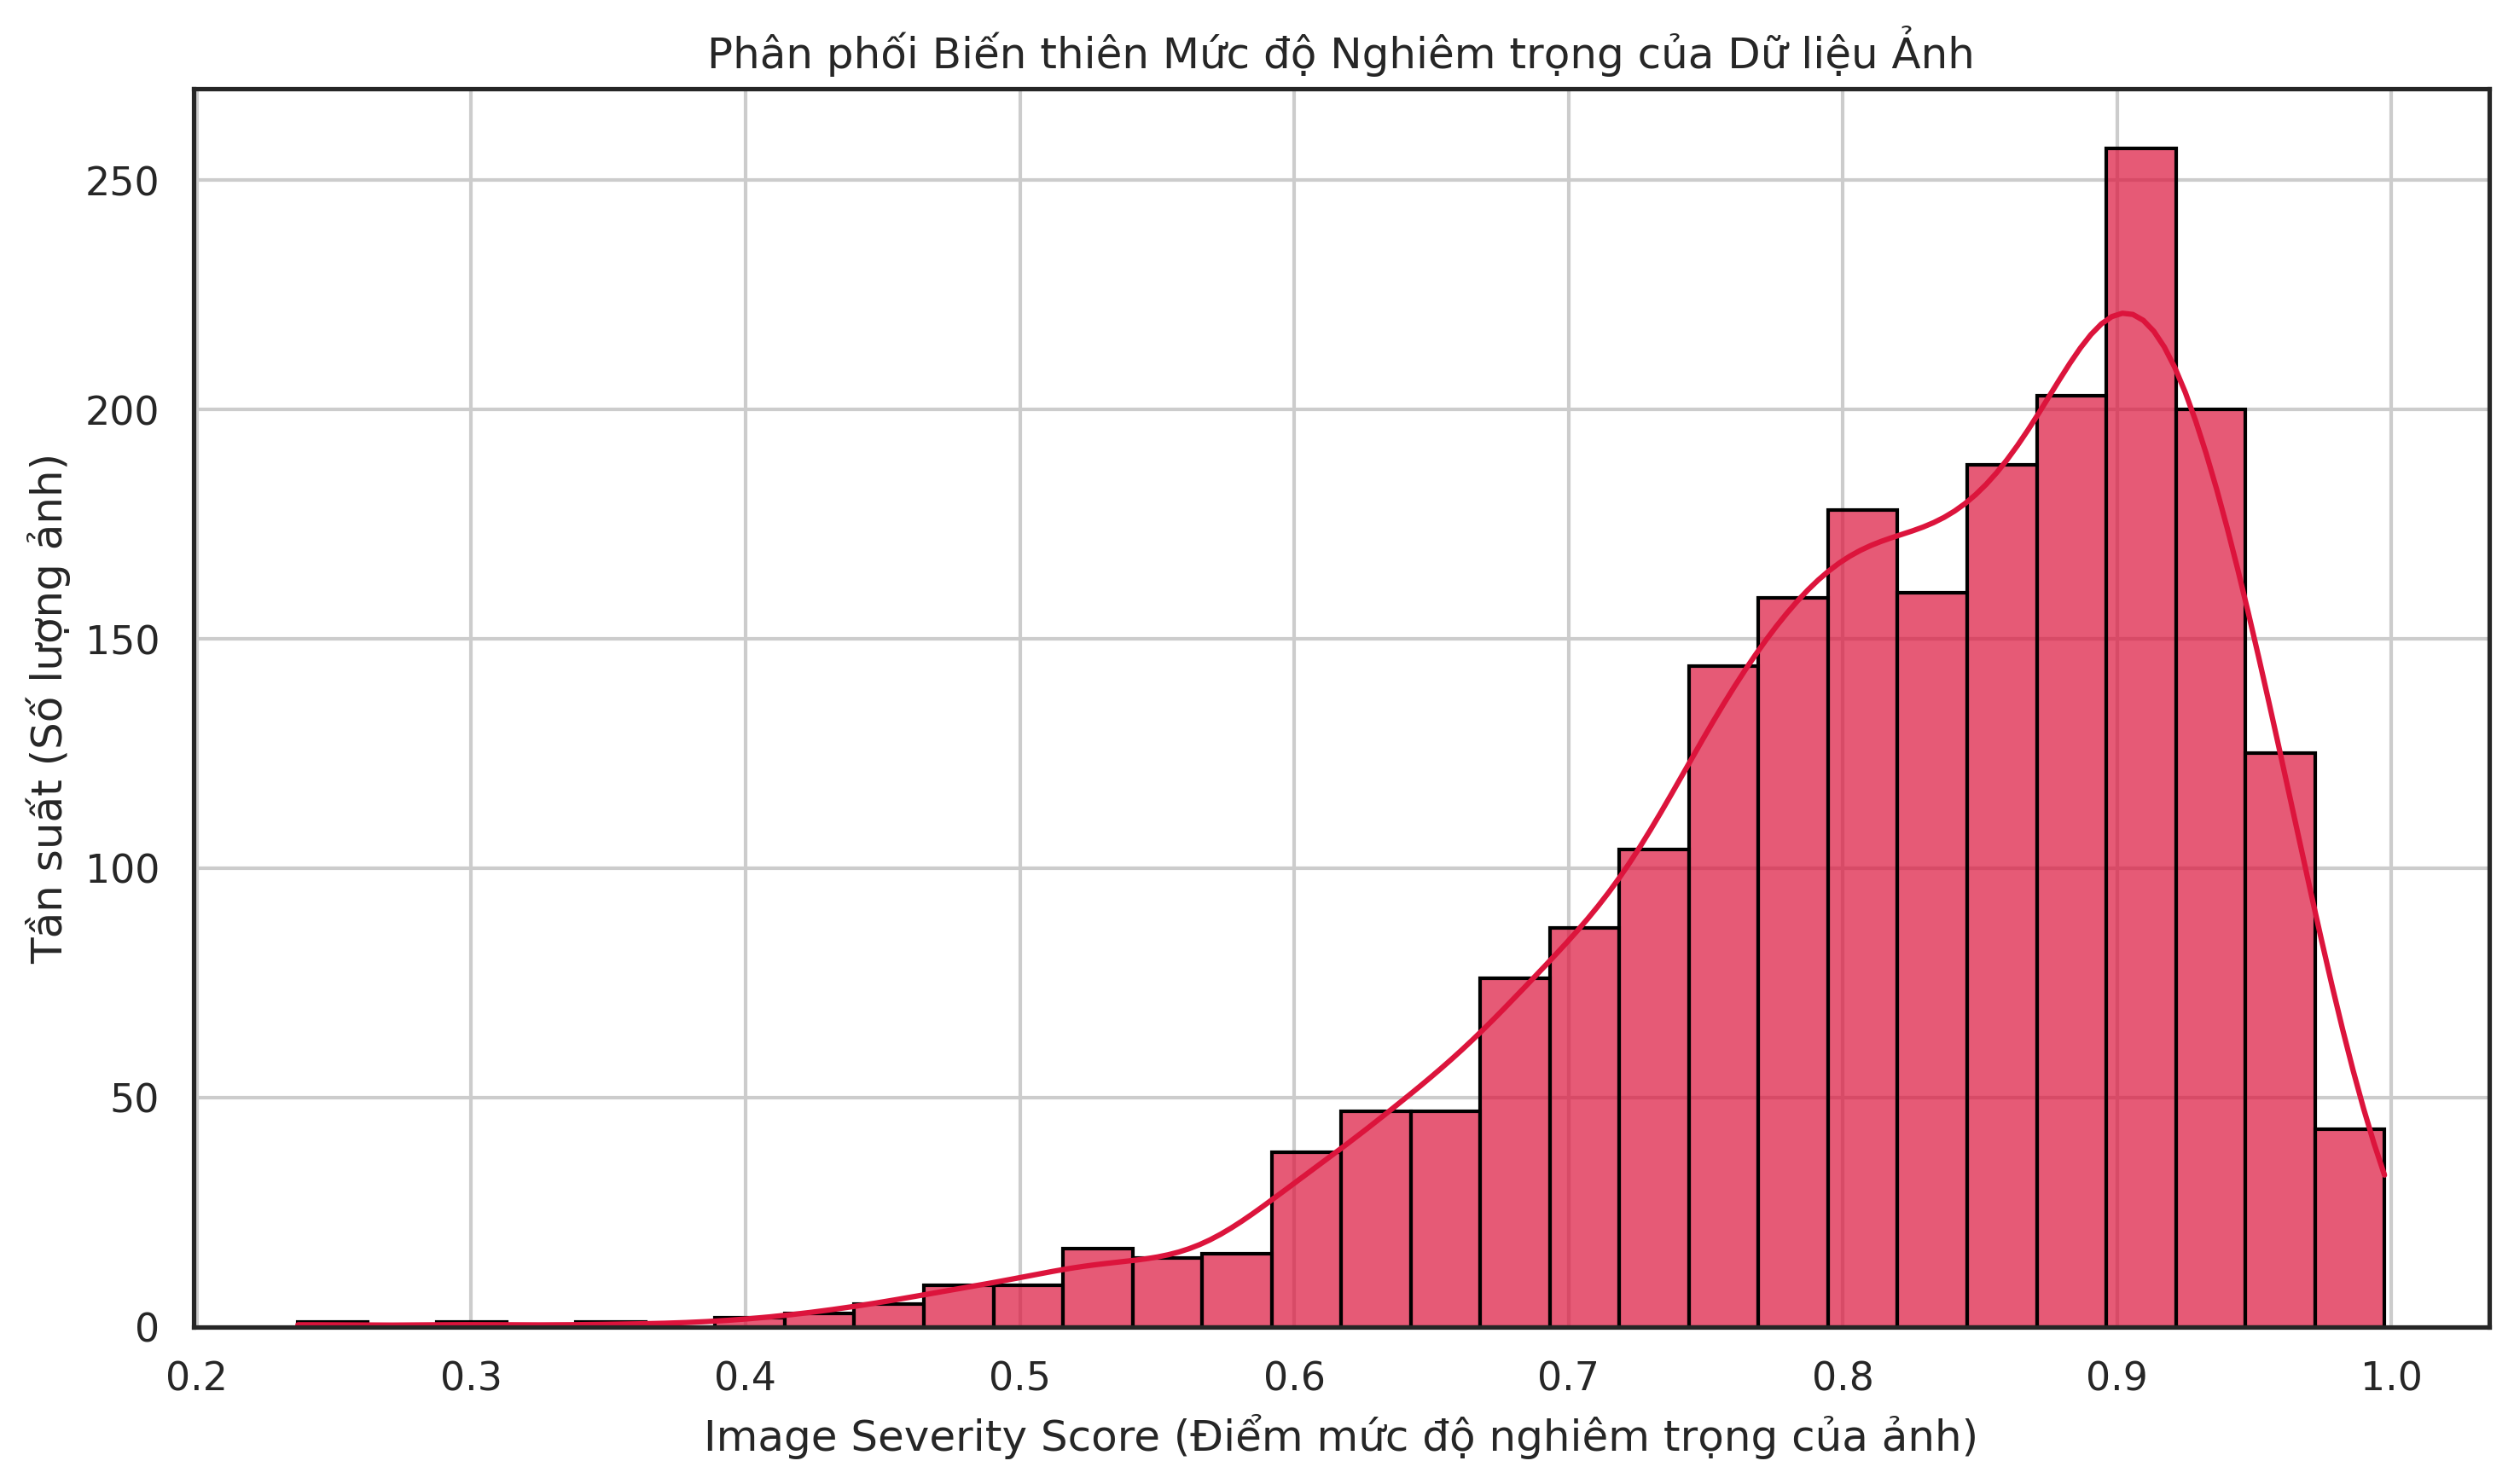
\includegraphics[width=\linewidth]{img/report/caitien/02_image_severity_distribution_improved.png}
        \caption{Phân bố độ nghiêm trọng ở mức ảnh}
      \end{figure}
  \end{columns}
  \small Ảnh tập trung mạnh ở vùng severity cao (xấp xỉ $0.75$--$0.95$, đỉnh quanh $0.88$--$0.92$), cho thấy độ khó là đặc tính phổ biến của tập dữ liệu.
\end{frame}

\begin{frame}{V-A.2 Hàm ý cho chiến lược huấn luyện}
  \small
  Phân bố lệch về vùng khó dẫn tới hai hàm ý:
  \begin{itemize}
    \item Huấn luyện ngẫu nhiên từ đầu dễ làm tối ưu dao động do gặp ảnh khó với tần suất cao khi đặc trưng lớp chưa ổn định.
    \item Độ khó không đến từ vài ngoại lệ, nên hướng cải thiện cần xử lý trực tiếp ba nguyên nhân gốc:
    \begin{itemize}
      \item texture cục bộ,
      \item boundary giữa lớp,
      \item quan hệ đồng xuất hiện/tiếp xúc giữa nguyên liệu.
    \end{itemize}
  \end{itemize}
\end{frame}

\subsection{Cải tiến BiSeNet}
\label{subsec:proposed_bisenet_rtb}

\begin{frame}{V-B. Kiến trúc BiSeNet cải tiến}
  \small
  Từ phân tích baseline, BiSeNet còn ba hạn chế chính:
  \begin{enumerate}
    \item thiếu biểu diễn texture cục bộ,
    \item thiếu mô hình hóa quan hệ giữa các lớp,
    \item thiếu giám sát trực tiếp tại vùng biên.
  \end{enumerate}
  \vspace{0.2em}
  Đề xuất mở rộng theo 3 thành phần nhẹ: \textit{Texture-aware Branch}, \textit{Relation GNN Module}, \textit{Boundary-aware Supervision}.
\end{frame}

\begin{frame}{V-B.1 Tổng quan kiến trúc đề xuất}
  \begin{figure}
    \centering
    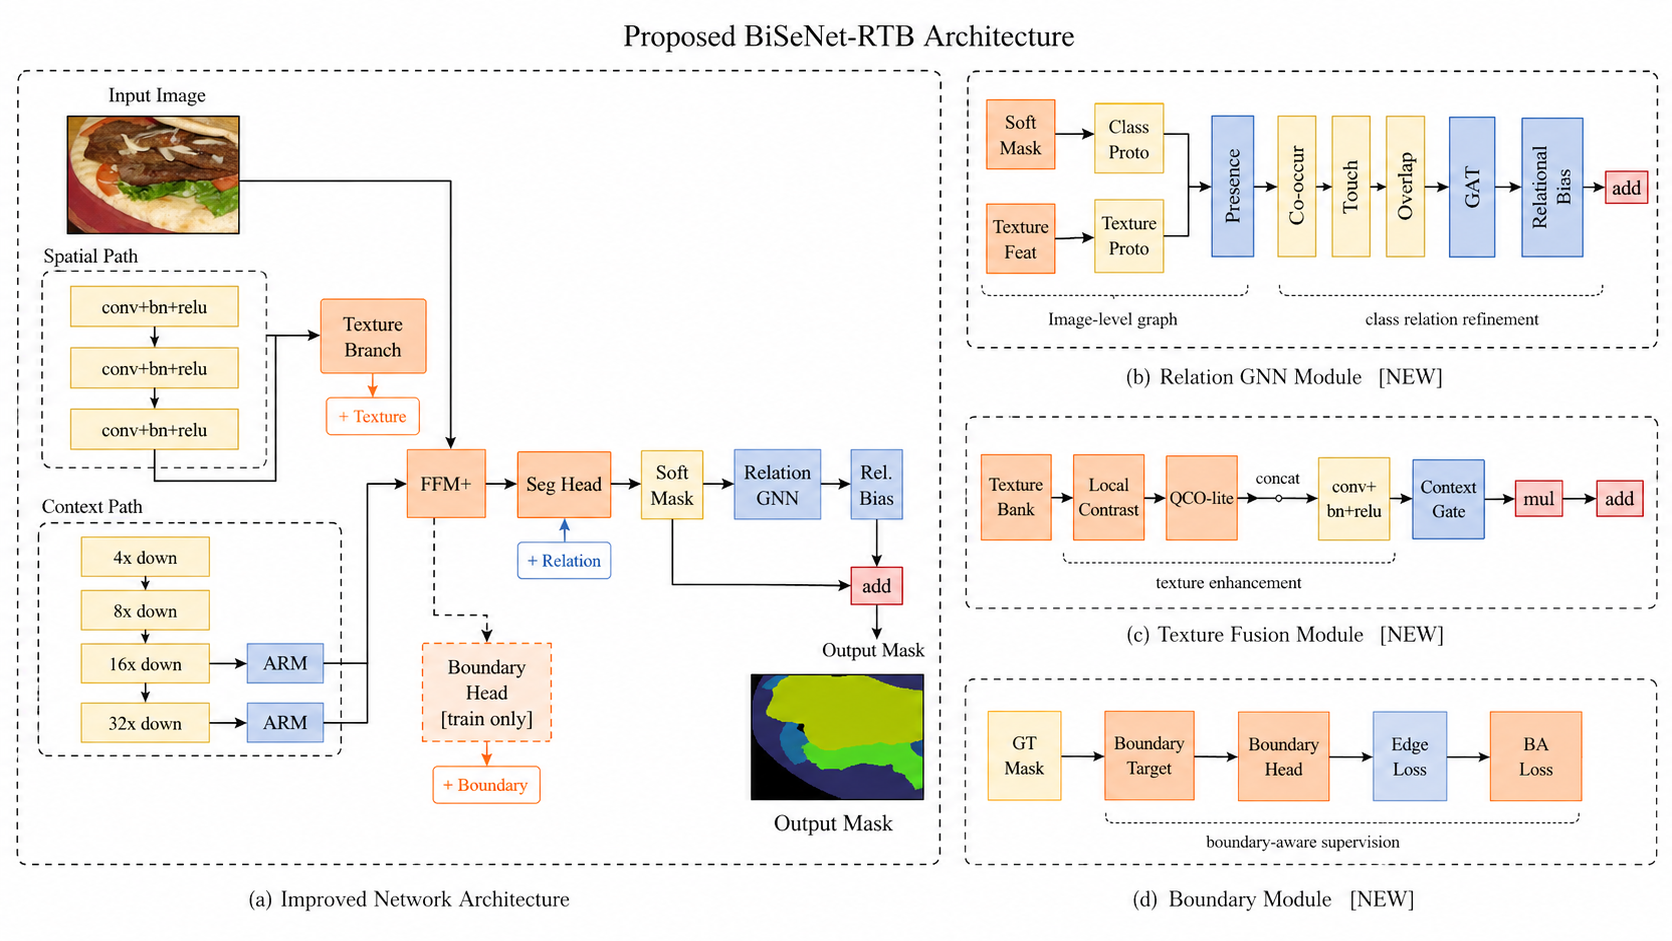
\includegraphics[width=0.6\linewidth]{img/report/caitien/proposed_bisenet_architecture.png}
    \caption{BiSeNet cải tiến với 3 thành phần bổ sung}
  \end{figure}
\end{frame}

\begin{frame}{V-B.2 Texture-aware Branch}
  \small
  Từ đặc trưng không gian $F_{sp}$:
  \[
    T = \phi_{\text{tex}}(F_{sp}), \qquad
    F_{sp}^{\text{tex}} = F_{sp} + \psi([F_{sp}, T]).
  \]
  \begin{itemize}
    \item $\phi_{\text{tex}}$: nhánh trích xuất cạnh nhỏ, tương phản cục bộ, cấu trúc bề mặt.
    \item $F_{sp}^{\text{tex}}$ được đưa vào Feature Fusion Module với Context Path.
  \end{itemize}
  \begin{block}{Mục tiêu}
    Giảm nhầm lẫn các lớp có hình thái tương tự nhưng khác texture (thịt, bánh, sốt, rau chế biến).
  \end{block}
\end{frame}

\begin{frame}{V-B.3 Relation GNN Module}
  \small
  Với logits sơ bộ $Y \in \mathbb{R}^{K \times H \times W}$, đặt:
  \[
    q_i(u) = \mathrm{softmax}(Y)_i(u), \qquad
    f_i = \frac{\sum_u q_i(u)F(u)}{\sum_u q_i(u)+\epsilon}.
  \]
  Nếu dùng texture feature $T$:
  \[
    \tau_i = \frac{\sum_u q_i(u)T(u)}{\sum_u q_i(u)+\epsilon}, \qquad
    x_i = [W_f f_i \, || \, W_t \tau_i \, || \, a_i].
  \]
  \[
    A = \mathrm{row\_norm}(\alpha A_{\text{cooc}} + \beta A_{\text{touch}} + \gamma A_{\text{overlap}}).
  \]
\end{frame}

\begin{frame}{V-B.4 Relation GNN: cập nhật và hiệu chỉnh logits}
  \small
  \[
    h_i^{(l+1)} = \sigma\!\left(\sum_{j \in \mathcal{N}(i)} A_{ij} W^{(l)} h_j^{(l)}\right),
    \qquad
    b_i = w_b^\top h_i^{(L)}.
  \]
  \[
    Y'_i(u) = Y_i(u) + \eta b_i.
  \]
  \begin{block}{Mục tiêu}
    Giảm lỗi có cấu trúc: sink class và nhầm lẫn giữa các lớp thường đồng xuất hiện/tiếp xúc.
  \end{block}
\end{frame}

\begin{frame}{V-B.3 Boundary-aware Supervision}
  \small
  Từ ground-truth mask $S$, sinh bản đồ biên:
  \[
    B = \mathrm{Dilate}(S) - \mathrm{Erode}(S), \qquad
    \hat{B} = \phi_{\text{bd}}(F_{sp}^{\text{tex}}).
  \]
  \[
    L_{\text{edge}} = \mathrm{WBCE}(\hat{B}, B) + \lambda_d L_{\text{Dice}}(\hat{B}, B).
  \]
  \[
    L_{\text{ba}} = -\frac{1}{|\Omega_b|}\sum_{u \in \Omega_b}\log p_{S(u)}(u).
  \]
  \begin{itemize}
    \item Boundary Head chỉ dùng khi train, suy luận vẫn giữ chi phí gần baseline.
    \item Tập trung giảm lỗi mask tràn biên, dính lớp và bỏ sót vùng nhỏ.
  \end{itemize}
\end{frame}

\begin{frame}{V-B.4 Loss tổng và vai trò từng thành phần}
  \small
  \[
    L_{\text{total}} =
    L_{\text{seg}}
    + \lambda_{\text{edge}}L_{\text{edge}}
    + \lambda_{\text{ba}}L_{\text{ba}}
    + \lambda_{\text{rel}}L_{\text{rel}}.
  \]
  \vspace{0.2em}
  \begin{itemize}
    \item \textbf{Texture-aware Branch:} Bổ sung texture cục bộ $\rightarrow$ giảm nhầm lớp bề mặt giống nhau.
    \item \textbf{Relation GNN:} Mô hình hóa đồng xuất hiện/tiếp xúc/chồng lấp $\rightarrow$ giảm sink class và lỗi có cấu trúc.
    \item \textbf{Boundary-aware Supervision:} Tăng giám sát biên $\rightarrow$ giảm tràn biên, dính lớp, bỏ sót vùng nhỏ.
  \end{itemize}
\end{frame}

\subsection{Kết quả}

\begin{frame}{V-C. Prior đồ thị lớp cho Relation GNN}
  \small
  \begin{columns}
    \column{0.4\textwidth}
    \begin{figure}
      \centering
      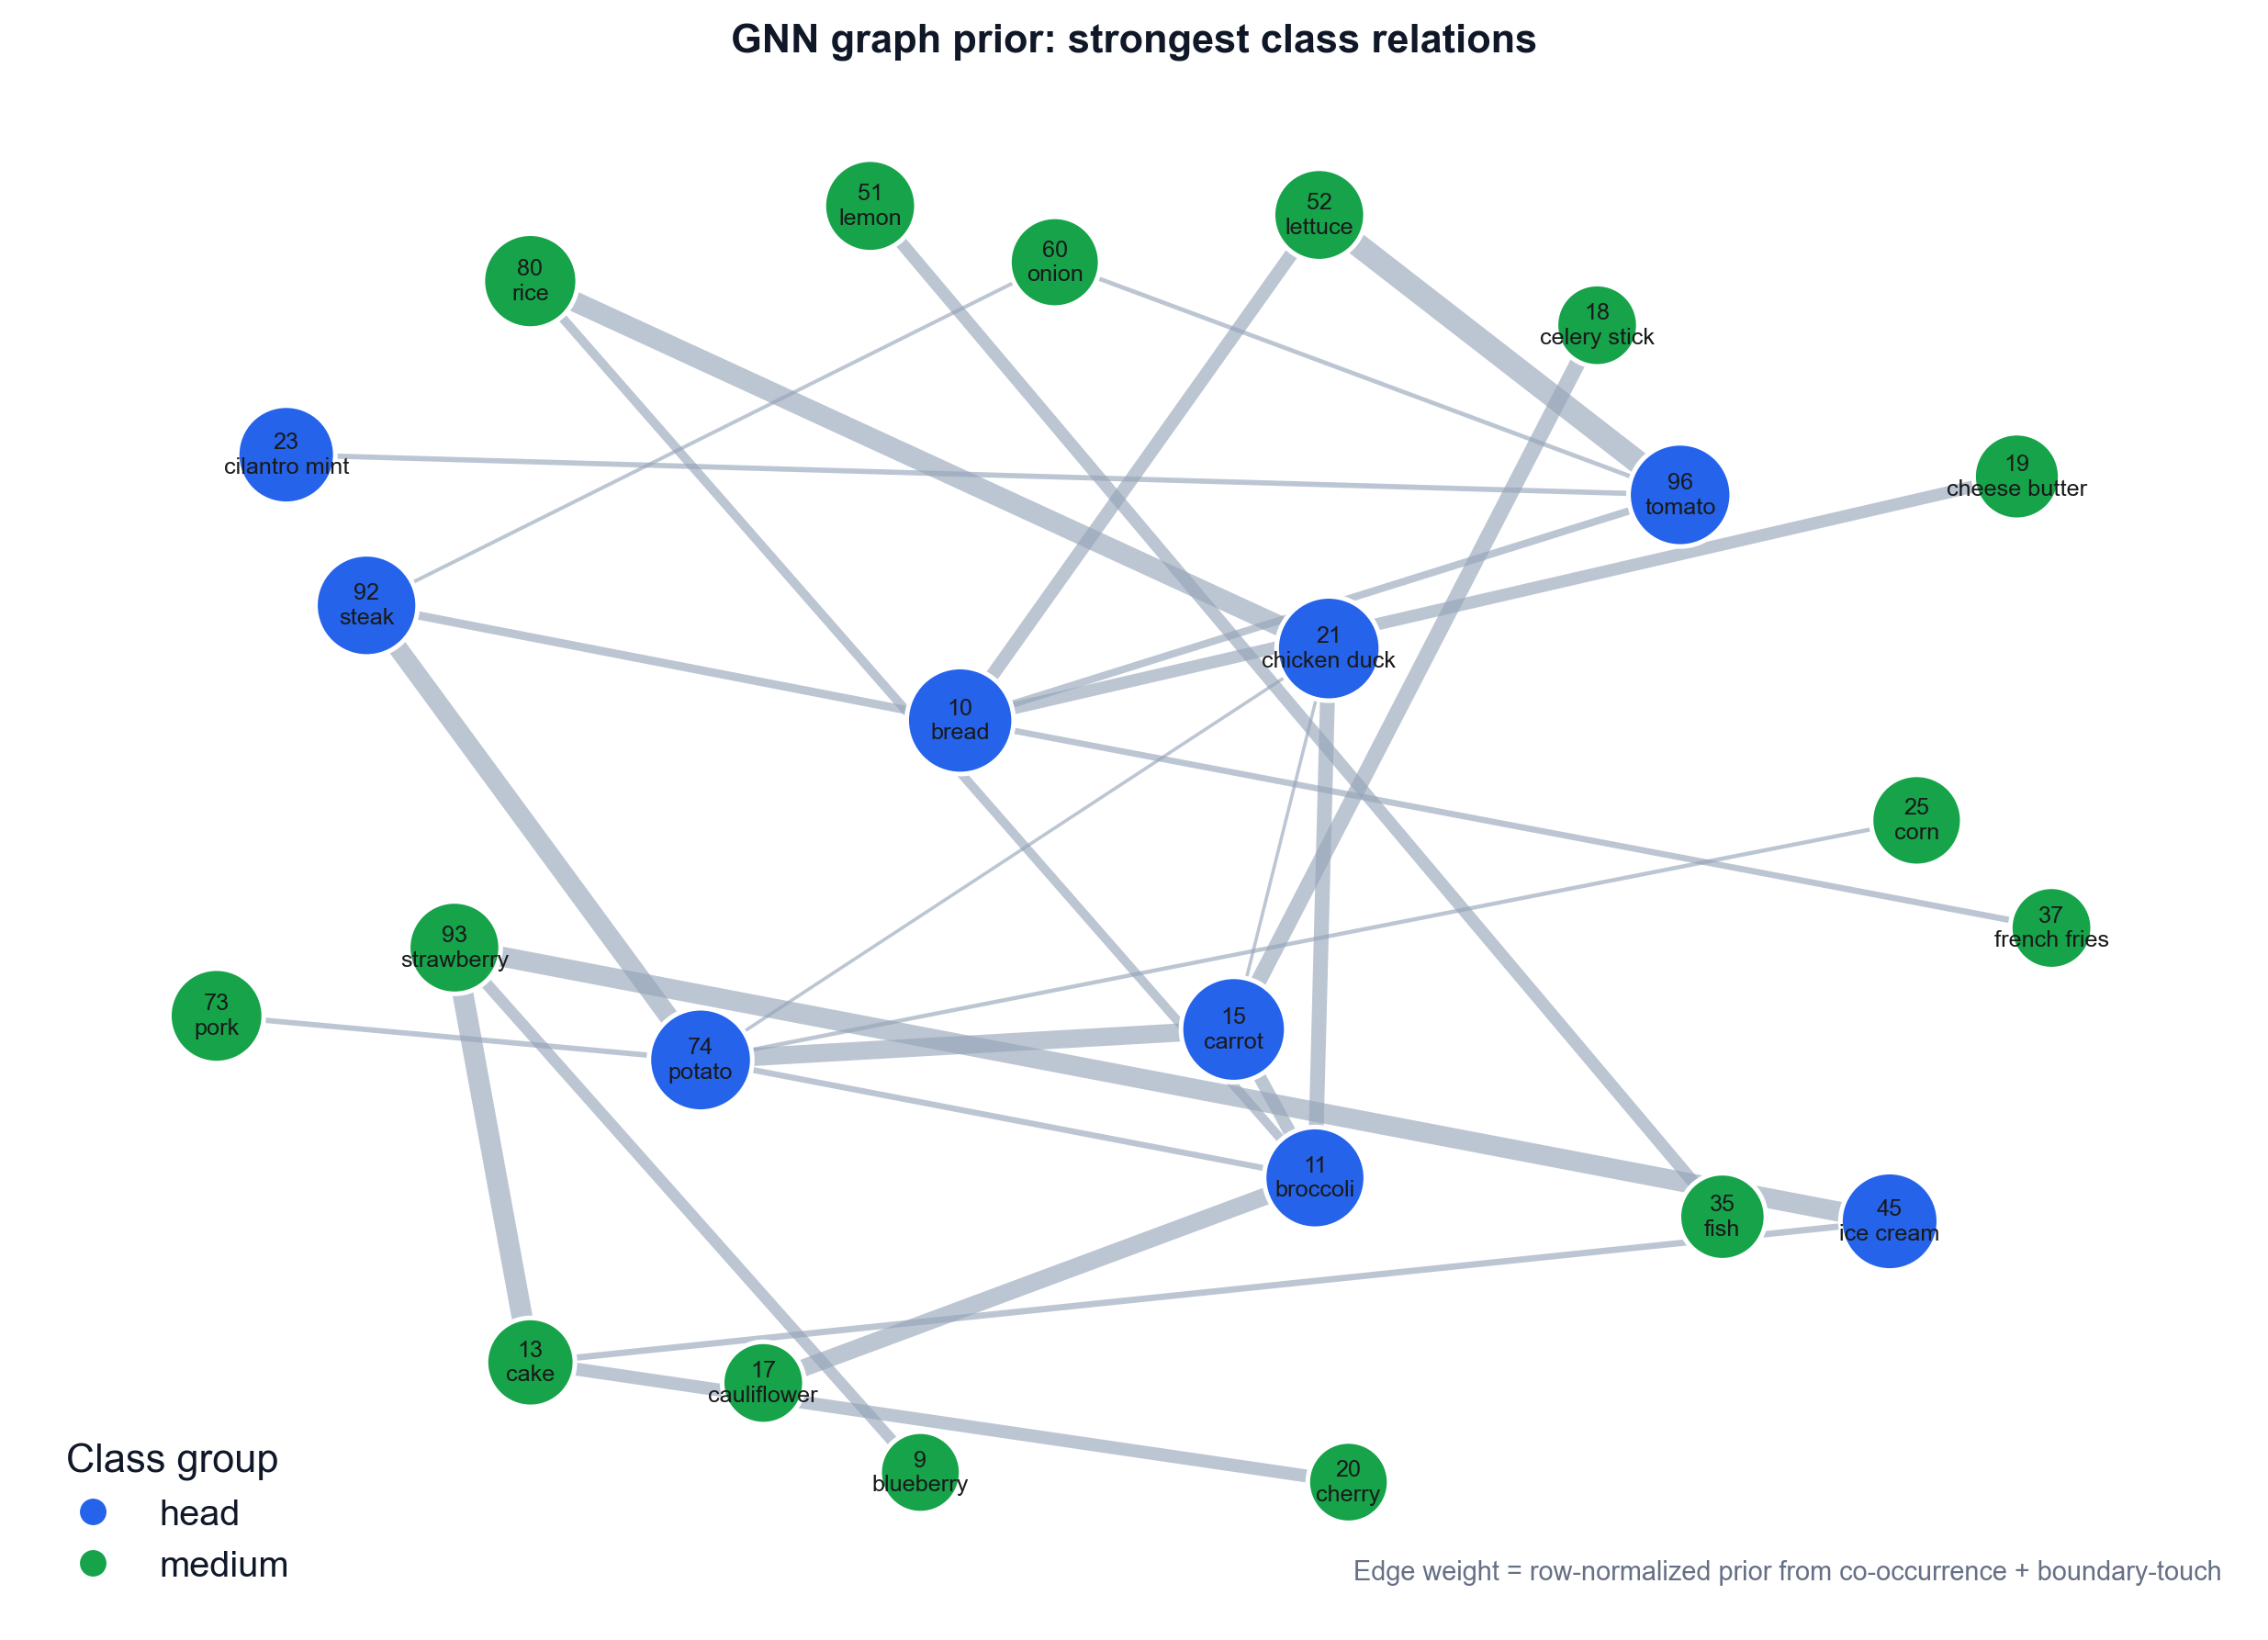
\includegraphics[width=0.7\linewidth]{img/report/caitien/plot/08_gnn_prior_top_edges_network.png}
      \caption{Các quan hệ lớp mạnh nhất}
    \end{figure}
    \column{0.4\textwidth}
    \begin{figure}
      \centering
      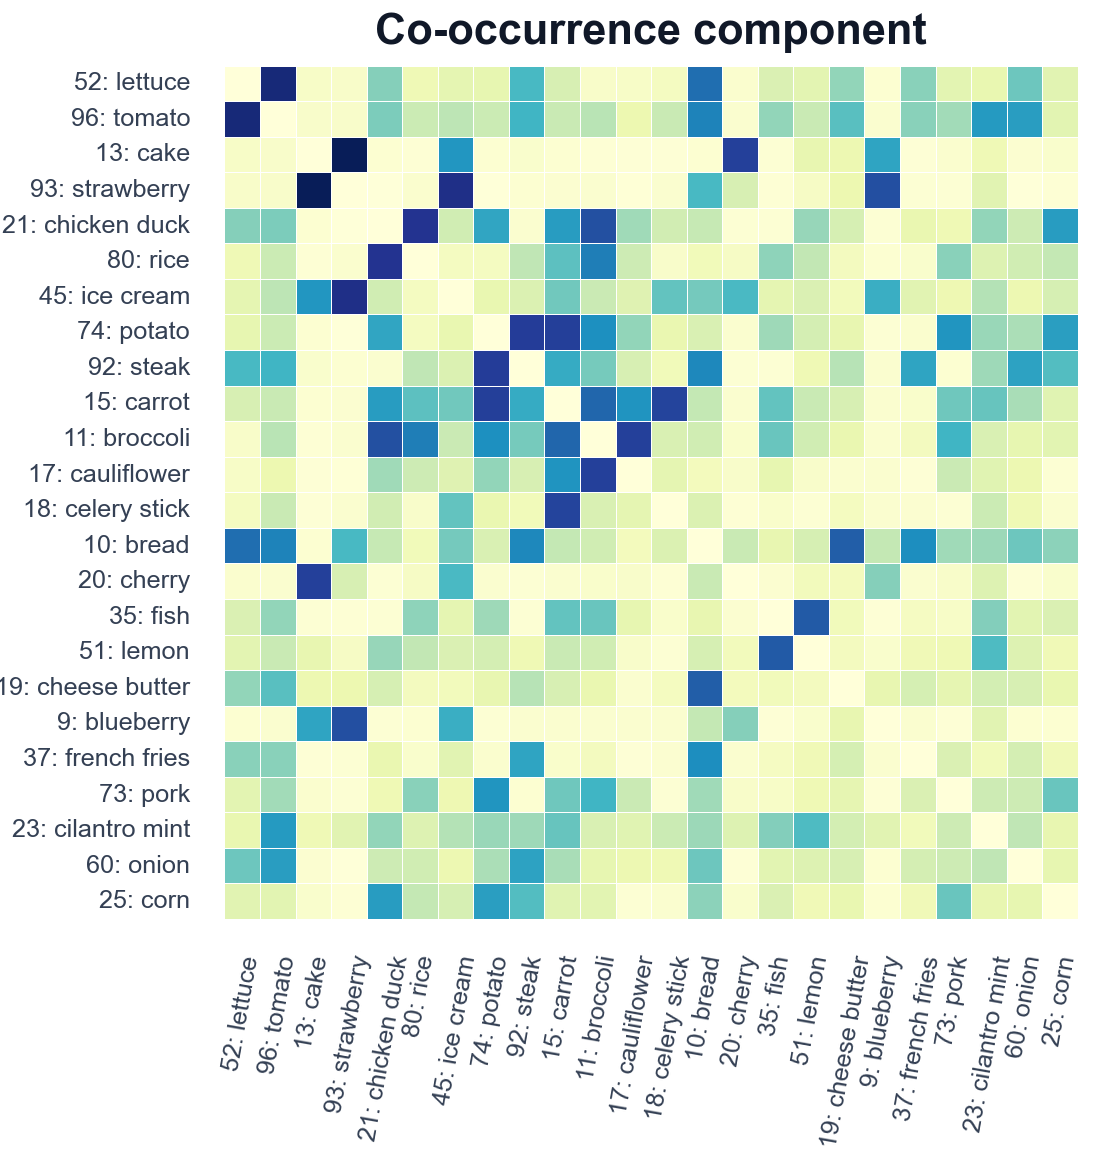
\includegraphics[width=0.7\linewidth]{img/report/caitien/plot/09_gnn_prior_components_heatmap.png}
      \caption{Heatmap đồng xuất hiện}
    \end{figure}
  \end{columns}
  \tiny Head classes như \texttt{bread}, \texttt{chicken duck}, \texttt{tomato}, \texttt{potato}, \texttt{broccoli} đóng vai trò nút liên kết mạnh, củng cố giả thuyết lỗi có cấu trúc theo ngữ cảnh món ăn.
\end{frame}

\begin{frame}{V-C. Diễn biến huấn luyện RTB/GNN}
  \begin{columns}
    \column{0.5\textwidth}
    \begin{figure}
      \centering
      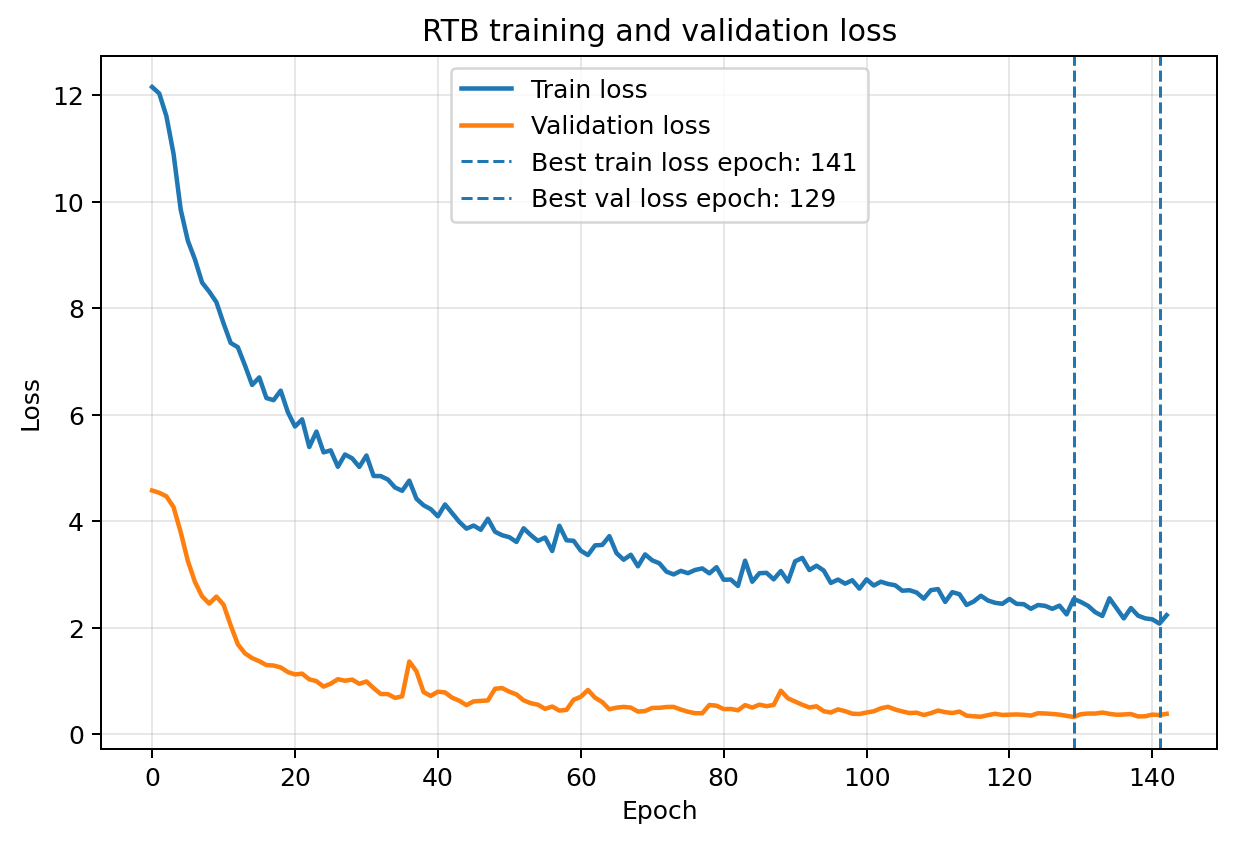
\includegraphics[width=\linewidth]{img/report/caitien/plot/rtb_best_loss.png}
      \caption{Train/Validation loss}
    \end{figure}
    \column{0.5\textwidth}
    \begin{figure}
      \centering
      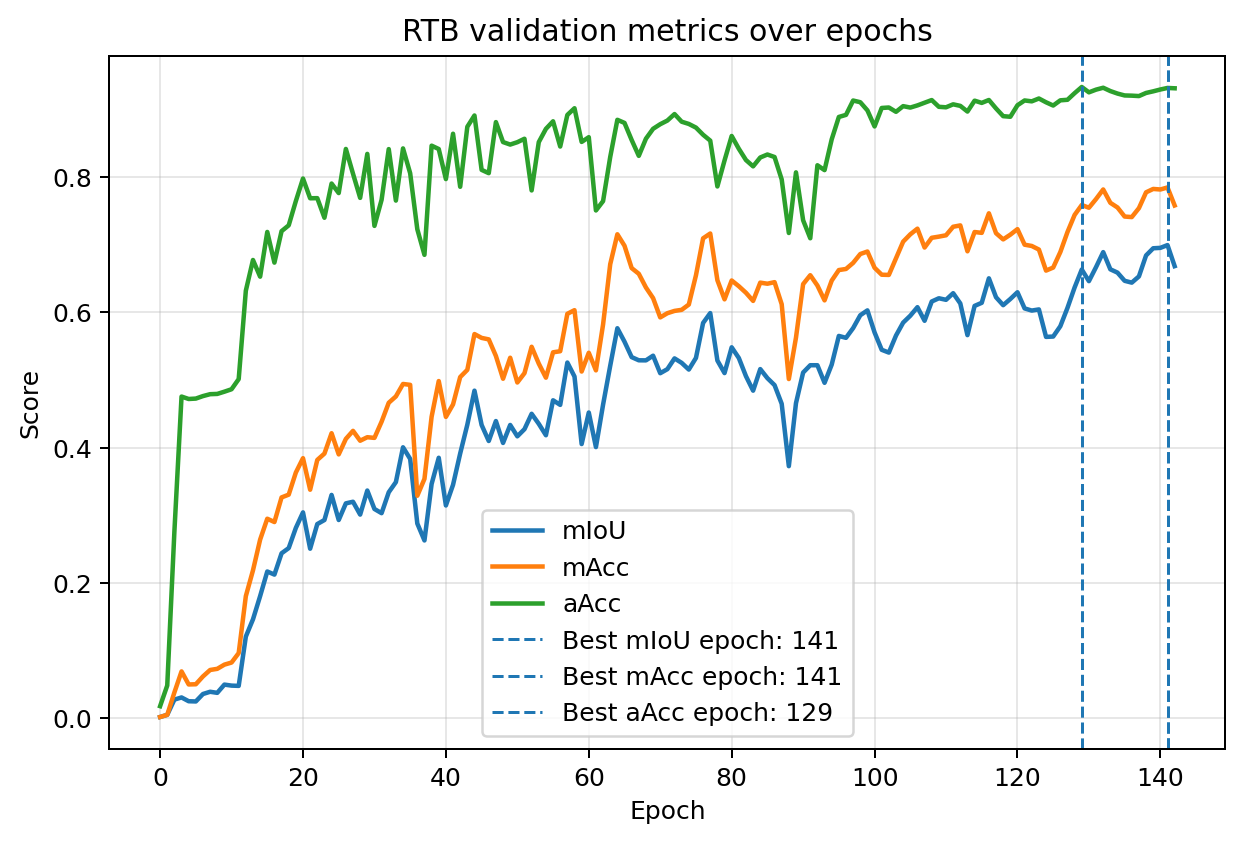
\includegraphics[width=\linewidth]{img/report/caitien/plot/rtb_best_metrics.png}
      \caption{Chỉ số validation theo epoch}
    \end{figure}
  \end{columns}
  \small Loss hội tụ ổn định; checkpoint tốt nhất theo val-loss ở epoch 129, còn mIoU/mAcc tốt nhất ở epoch 141.
\end{frame}

\begin{frame}{V-C. Lỗi hiện diện lớp}
  \begin{columns}
    \column{0.5\textwidth}
    \begin{block}{Nhận xét}
      \small
      \begin{itemize}
        \item Lỗi dương giả giảm rõ rệt sau khi bổ sung prior GNN và các ràng buộc biên.
        \item Mô hình kiểm soát tốt hơn việc dự đoán lớp không xuất hiện trong ảnh.
      \end{itemize}
    \end{block}
    \column{0.5\textwidth}
    \begin{figure}
      \centering
      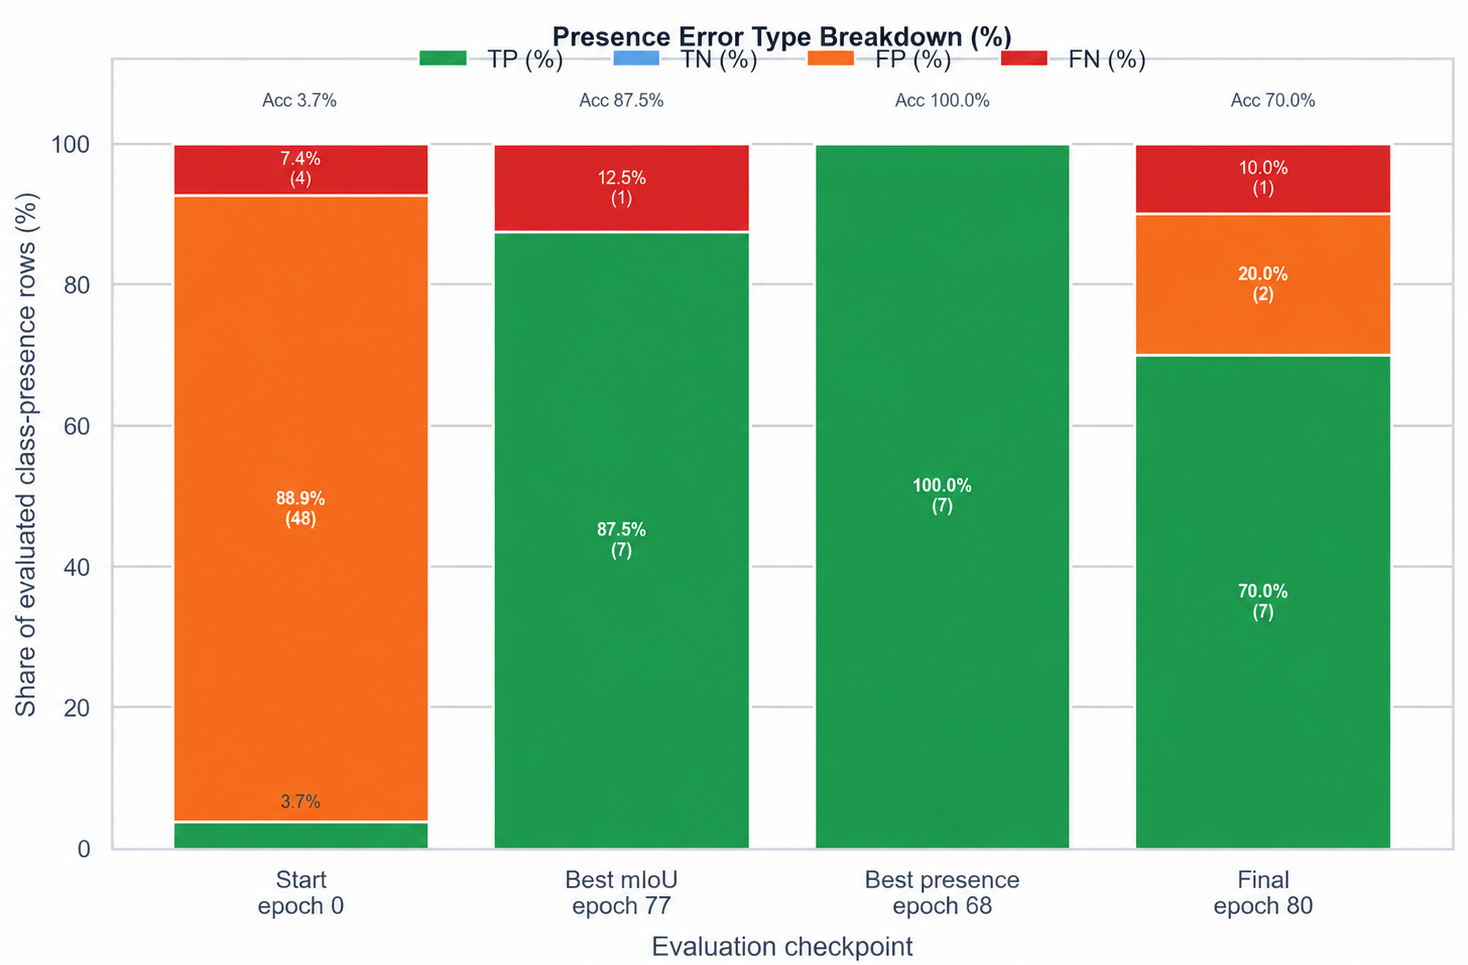
\includegraphics[width=\linewidth]{img/report/caitien/plot/presence error.png}
      \caption{Phân tích lỗi presence}
    \end{figure}
  \end{columns}
\end{frame}
